\documentclass[a4paper, article, oneside, UKenglish]{memoir}


%% Encoding
\usepackage[utf8]{inputenx} % Source code
\usepackage[T1]{fontenc}    % PDF

%% Fonts and typography
\usepackage{lmodern}           % Latin Modern Roman
\usepackage[scaled]{beramono}  % Bera Mono (Bitstream Vera Sans Mono)
\renewcommand{\sfdefault}{phv} % Helvetica
\usepackage[final]{microtype}  % Improved typography
\pretitle{\begin{center}\LARGE\sffamily\bfseries}                    % Title
\renewcommand{\abstractnamefont}{\sffamily\bfseries}                 % Abstract
\renewcommand*{\chaptitlefont}{\Large\bfseries\sffamily\raggedright} % Chapter
\setsecheadstyle{\large\bfseries\sffamily\raggedright}               % Section


%% Mathematics
\usepackage{amssymb}   % Extra symbols
\usepackage{amsthm}    % Theorem-like environments
\usepackage{thmtools}  % Theorem-like environments
\usepackage{mathtools} % Fonts and environments for mathematical formuale
\usepackage{mathrsfs}  % Script font with \mathscr{}

%% Miscellanous
\usepackage{graphicx}  % Tool for images
\usepackage{subcaption}
\usepackage{float}
\usepackage{gensymb}
\usepackage{babel}     % Automatic translations
\usepackage{csquotes}  % Quotes
\usepackage{textcomp}  % Extra symbols
\usepackage{listings}  % Typesetting code
\usepackage[left=2cm, right=2cm, top=2cm]{geometry}

%% Bibliography
\usepackage[backend = biber, style = alphabetic]{biblatex}
%\addbibresource{<NAME OF BIBLIOGRAPY FILE>.bib}


%% Cross references
\usepackage{varioref}
\usepackage{hyperref}
\urlstyle{sf}
\usepackage[nameinlink, capitalize, noabbrev]{cleveref}


%% Theorem-like environments
\declaretheorem[style = plain, numberwithin = chapter]{theorem}
\declaretheorem[style = plain,      sibling = theorem]{corollary}
\declaretheorem[style = plain,      sibling = theorem]{lemma}
\declaretheorem[style = plain,      sibling = theorem]{proposition}
\declaretheorem[style = definition, sibling = theorem]{definition}
\declaretheorem[style = definition, sibling = theorem]{example}
\declaretheorem[style = remark,    numbered = no]{remark}


%% Delimiters
\DeclarePairedDelimiter{\p}{\lparen}{\rparen}   % Parenthesis
\DeclarePairedDelimiter{\set}{\lbrace}{\rbrace} % Set
\DeclarePairedDelimiter{\abs}{\lvert}{\rvert}   % Absolute value
\DeclarePairedDelimiter{\norm}{\lVert}{\rVert}  % Norm


%% Operators
\DeclareMathOperator{\im}{im}
\DeclareMathOperator{\rank}{rank}
\DeclareMathOperator{\E}{E}
\DeclareMathOperator{\Var}{Var}
\DeclareMathOperator{\Cov}{Cov}


%% New commands for sets
\newcommand{\N}{\mathbb{N}}   % Natural numbers
\newcommand{\Z}{\mathbb{Z}}   % Integers
\newcommand{\Q}{\mathbb{Q}}   % Rational numbers
\newcommand{\R}{\mathbb{R}}   % Real numbers
\newcommand{\C}{\mathbb{C}}   % Complex numbers
\newcommand{\A}{\mathbb{A}}   % Affine space
\renewcommand{\P}{\mathbb{P}} % Projective space


%% New commands for vectors
\renewcommand{\a}{\mathbf{a}}
\renewcommand{\b}{\mathbf{b}}
\renewcommand{\c}{\mathbf{c}}
\renewcommand{\v}{\mathbf{v}}
\newcommand{\w}{\mathbf{w}}
\newcommand{\x}{\mathbf{x}}
\newcommand{\y}{\mathbf{y}}
\newcommand{\z}{\mathbf{z}}
\newcommand{\0}{\mathbf{0}}
\newcommand{\1}{\mathbf{1}}


%% Miscellanous
\renewcommand{\qedsymbol}{\(\blacksquare\)}


\title{IN5520/IN9520 Mandatory term project 2018 – Part II \\ Feature evaluation and classification}
\author{Francisco Jose Nava Lujan \\ User name: francijn}


\begin{document}


\maketitle


\begin{abstract}
\noindent
The present work discusses the implementation of various methods for feature extraction and classification of image data. A visual representation of GLCM images describing the data was analyzed in order to determine useful features for classification, and a subset of particular features was selected to implement a better classifier. A multivariate Gaussian density model was then implemented using the data collected from features of a training set. Finally, evaluation of performance was done on testing data using the information obtained.
\end{abstract}

\chapter{Choosing GLCM images to work with}
The first task is to choose the most appropriate features to extract from the original textures. In \cref{fig:m1t}, we can see the training set, labeled for future reference. 
   \begin{figure}[h]
     \begin{center}
       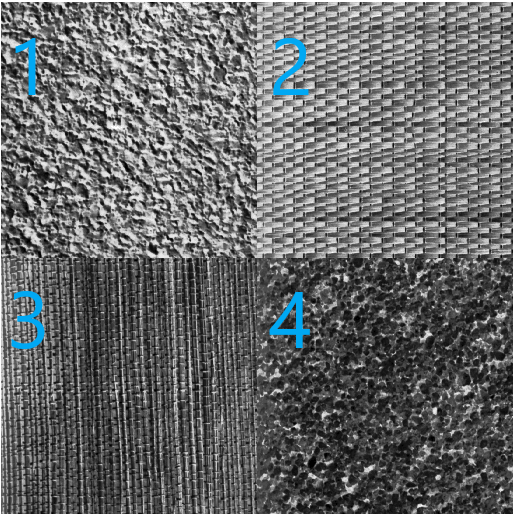
\includegraphics[width=0.5\linewidth]{./images/mosaic1_train.png}
     \end{center}
  \caption{mosaic1\_train}
  \label{fig:m1t}
\end{figure}

The goal is to classify each one of the four textures shown. To do this, we can look at the GLCM (Gray Level Co-occurrence Matrix) of each texture with different step directions as images, and try to determine which directions give us useful information. As we can see in the original training set, the textures have mostly horizontal or vertical patterns, so let's start by analyzing GLCM with step directions of 0 and 90 degrees. This GLCM images are shown in \cref{fig:t1glcm}, \cref{fig:t2glcm}, \cref{fig:t3glcm}, \cref{fig:t4glcm}.

\begin{figure}
  \centering
  \begin{subfigure}[b]{0.45\linewidth}
    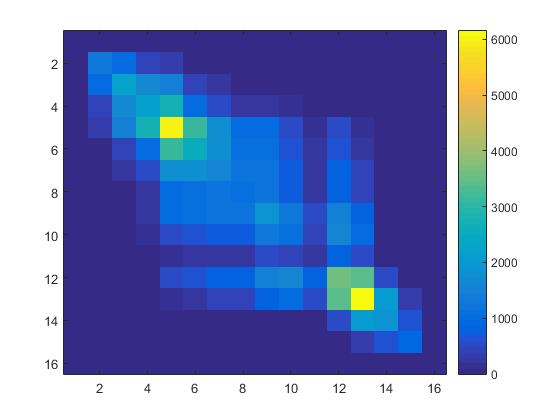
\includegraphics[width=\linewidth]{./images/tx1-0.png}
    \caption{$\theta$=0}
  \end{subfigure}
  \begin{subfigure}[b]{0.45\linewidth}
    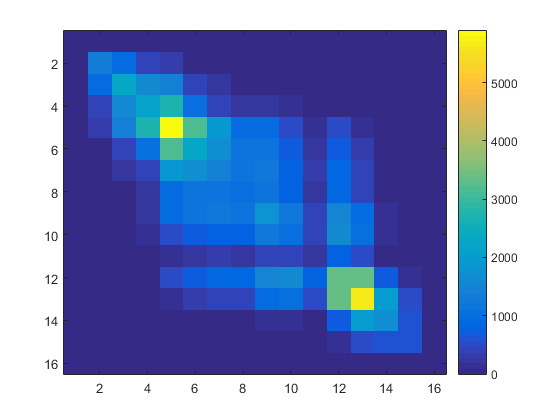
\includegraphics[width=\linewidth]{./images/tx1-90.png}
    \caption{$\theta$=90}
  \end{subfigure}
  \caption{For mosaic1\_train texture 1 : d = 1, $\theta$=0 and 90.}
  \label{fig:t1glcm}
\end{figure}

\begin{figure}
  \centering
  \begin{subfigure}[b]{0.45\linewidth}
    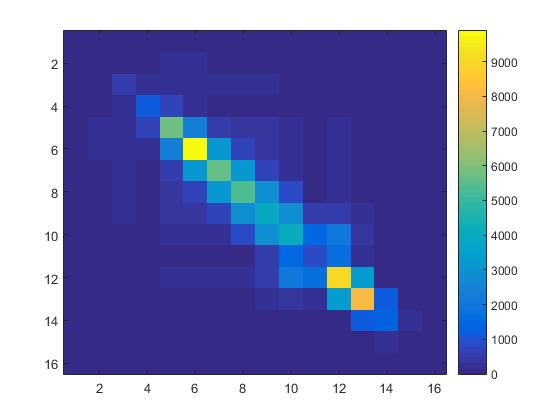
\includegraphics[width=\linewidth]{./images/tx2-0.png}
    \caption{$\theta$=0}
  \end{subfigure}
  \begin{subfigure}[b]{0.45\linewidth}
    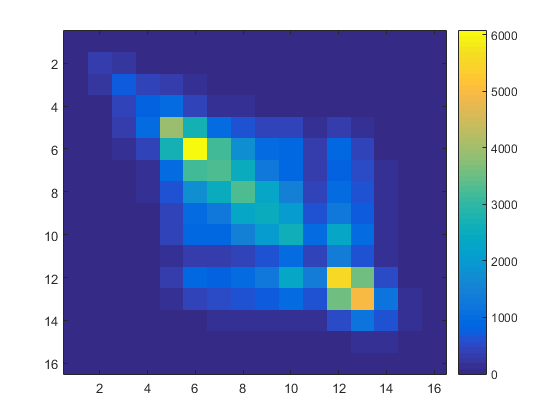
\includegraphics[width=\linewidth]{./images/tx2-90.png}
    \caption{$\theta$=90}
  \end{subfigure}
  \caption{For mosaic1\_train texture 2 : d = 1, $\theta$=0 and 90.}
  \label{fig:t2glcm}
\end{figure}

\begin{figure}
  \centering
  \begin{subfigure}[b]{0.45\linewidth}
    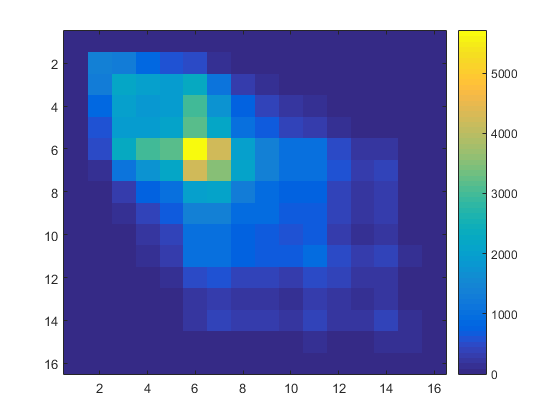
\includegraphics[width=\linewidth]{./images/tx3-0.png}
    \caption{$\theta$=0}
  \end{subfigure}
  \begin{subfigure}[b]{0.45\linewidth}
    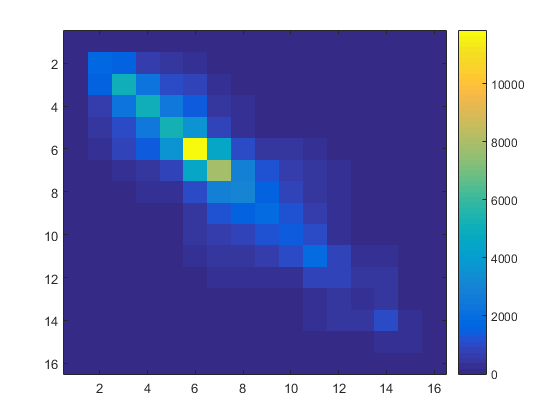
\includegraphics[width=\linewidth]{./images/tx3-90.png}
    \caption{$\theta$=90}
  \end{subfigure}
  \caption{For mosaic1\_train texture 3 : d = 1, $\theta$=0 and 90.}
  \label{fig:t3glcm}
\end{figure}

\begin{figure}
  \centering
  \begin{subfigure}[b]{0.45\linewidth}
    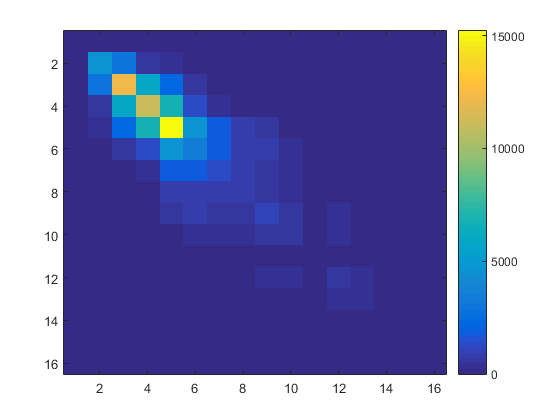
\includegraphics[width=\linewidth]{./images/tx4-0.png}
    \caption{$\theta$=0}
  \end{subfigure}
  \begin{subfigure}[b]{0.45\linewidth}
    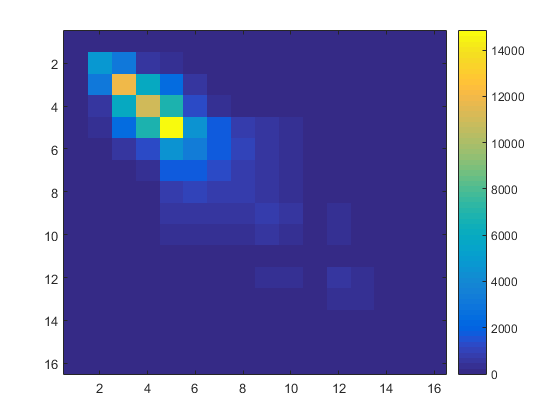
\includegraphics[width=\linewidth]{./images/tx4-90.png}
    \caption{$\theta$=90}
  \end{subfigure}
  \caption{For mosaic1\_train texture 4 : d = 1, $\theta$=0 and 90.}
  \label{fig:t4glcm}
\end{figure}

We can see that, for texture 2 and 3 (textures with horizontal and vertical patterns), the GLCM images are rather different, and that the information is found mostly in the matrix diagonal. For texture 1 and 4, since the texture spread is mostly random, or not following a particular pattern, the matrices are very similar for 0 and 90 degrees. We can expect the same to happen with the rest of the step directions for those two textures. Therefore, we have selected the GLCM matrices to be used for feature extraction. \\
\chapter{Discussing new features by subdividing the GLCM matrices}

To extract features from these matrices, a selection of useful data has to be obtained. As I have mentioned earlier, most of the information is given by the matrix diagonal, and not very much outside of the diagonal. If we divide the matrices into four quadrants, we can see the percentage of relevance of each quadrant and use this information as features for classification. Quadrant 1 (q1) is the top-left part of the matrix, q2 is the top-right, and so on. Based on the information of each quadrant we can obtain this percentage of relevance. Since the GLCM is a symmetric matrix, q2 and q3 will carry the same significance, so we can get rid of one of those quadrants as to not have repeated information in our analysis. Since this quadrants don't really contribute much information to the analysis anyway, I've decided to work only with q1 and q4 of the GLCMs as subsets of features to analyze. The code to extract these features from a GLCM is given by the following function, also found under the path \textit{./my\_funcs/q\_features.m}:

\lstset{language=Matlab}
\begin{lstlisting}[frame=single]  % Inicia el bloque de código

function [ q1, q4 ] = q_features( GLCM )
m = GLCM / sum(GLCM(:));

q1 = sum(sum(m(1:8,1:8)));
% q2 = sum(sum(m(1:8,9:16)));
% q3 = sum(sum(m(9:16,1:8));
q4 = sum(sum(m(9:16,9:16)));
end


\end{lstlisting}

Having looked at the data collected by this feature extraction function, only two quadrants per GLCM are enough to distiguish between the four textures. Since we're analyzing two directions, and two quadrants each, we will have a total of four feature elements in each feature vector.

\chapter{Selecting and implementing the best features from the GLCM matrices}

To implement this subset of features, a sliding window of size 31x31 was used in the image mosaic1\_train. To do this, first it is necesary to scale the value of gray-levels in the image to have 16 different levels (1-16). This is done by the next function, also found under the path \textit{./my\_funcs/my\_quantizer.m}:

\lstset{language=Matlab}
\begin{lstlisting}[frame=single]  % Inicia el bloque de código

function [ r1 ] = my_quantizer( x )
% Quantizing the image to 16 Gray Levels
for i = 1:numel(x)
    if (x(i)>=0 && x(i)<=15)
        x(i) = 1;
    elseif (x(i) >=16 && x(i)<=31)
        x(i) = 2;
    elseif (x(i)>=32 && x(i)<=47)
        x(i) = 3;
    elseif (x(i)>=48 && x(i)<=63)
        x(i) = 4;
    elseif (x(i)>=64 && x(i)<=79)
        x(i) = 5;
    elseif (x(i)>=80 && x(i)<=95)
        x(i) = 6;
    elseif (x(i)>=96 && x(i)<=111)
        x(i) = 7;
    elseif (x(i)>=112 && x(i)<=127)
        x(i) = 8;
    elseif (x(i)>=128 && x(i)<=143)
        x(i) = 9;
    elseif (x(i)>=144 && x(i)<=159)
        x(i) = 10;
    elseif (x(i)>=160 && x(i)<=175)
        x(i) = 11;
    elseif (x(i)>=176 && x(i)<=191)
        x(i) = 12;
    elseif (x(i)>=192 && x(i)<=207)
        x(i) = 13;
    elseif (x(i)>=208 && x(i)<=223)
        x(i) = 14;
    elseif (x(i)>=224 && x(i)<=239)
        x(i) = 15;
    elseif (x(i)>=240 && x(i)<=255)
        x(i) = 16;
    end
end
r1 = x;
end

\end{lstlisting}

Since the resulting feature images are calculated using sliding windows, they will be padded compared to the original image. We're using a sliding window of 31x31, meaning that the original image of size 512x512 will have only 482x482 resulting values. For further calculations, we adjust the training mask to this size using the next code, found in \textit{./main.m}:

\begin{lstlisting}[basicstyle=\small, frame=single]  % Inicia el bloque de código

num_classes = 4;
num_features = 4; 
dirs = 2; % We will use 2 directions, namely 0 and 90 degrees
windowSize = 31;
sowC = ceil(windowSize/2);
sowF = floor(windowSize/2);
GL = 16;

load('mosaic1_train.mat');
load('training_mask.mat');
% Padding on mask to match feature image size
train_msk = training_mask(sowC:end-sowF, sowC:end-sowF);
[tm_r, tm_c] = size(train_msk);
% Total classified pixels
totalnz = sum(sum(train_msk ~= 0));
% Number of pixels for each class
nof = zeros(1,num_classes);
for i = 1:num_classes
    nof(i) = sum(sum(train_msk == i));
end

train_img = zeros(tm_r, tm_c, num_features);
% Adjusting to 16 gray-levels
mos1 = my_quantizer(mosaic1_train);

\end{lstlisting}

Once we have the matrices where we will store the features, we proceed to calculate them using the sliding window. I have recycled some code used in the first mandatory project to do this. The central code for this extraction can be seen in the following function, also found in \textit{./my\_funcs/my\_features.m} (I added a progress bar in this code because it takes some time to run; it is helpful to see the progress of these calculations):

\begin{lstlisting}[frame=single]

function [ Q ] = my_features( x, sow, d, theta, nof )
f = waitbar(0,'1','Name','Extracting features...',...
    'CreateCancelBtn','setappdata(gcbf,''canceling'',1)');
setappdata(f,'canceling',0);
sowC = ceil(sow/2);
sowF = floor(sow/2);
% Initializing feature matrices
[n, m] = size(x(sowC:end-sowF, sowC:end-sowF));
Q = zeros(n, m, nof);
auxQ = zeros(1,nof);
step = 0;
steps = n * m;
for row = 1:size(Q,1)
    for col = 1:size(Q,2)
	% Calculation of GLCM
        newGL = my_glcm(x(row:row+(sow-1),col:col+(sow-1)), 16, d, theta); 
	% Feature extraction for q1 and q4, for one particular direction
        [auxQ(1), auxQ(2)] = q_features(newGL); 
        Q(row,col,:) = auxQ(:);
        step = step + 1;
        if getappdata(f,'canceling')
            break
        end
        waitbar(step/steps,f,sprintf('%.2f',(step/steps)*100))
    end
end
delete(f)
end

\end{lstlisting}

For the sake of documentation, the following code is used to calculate GLCM. Since this function is used in the feature extraction, I found it useful to include it, and it is also found under \textit{./my\_funcs/my\_glcm.m}:

\begin{lstlisting}[frame=single]  % Inicia el bloque de código

function [r1, r2] = my_glcm( x, GL, d, theta )
% Initializing GLCM matrix
r1 = zeros(GL,GL);
r2 = x;
if theta == 0
    for row = 1:size(x,1)
        for col = 1:size(x,2)-d
            r1(x(row,col),x(row,col+d)) = r1(x(row,col),x(row,col+d)) + 1;
        end
    end
elseif theta == 90
    for row = d+1:size(x,1)
        for col = 1:size(x,2)
            r1(x(row,col),x(row-d,col)) = r1(x(row,col),x(row-d,col)) + 1;
        end
    end
end
% Make symmetric
r1 = r1 + r1.';
% Return quantized image
r2 = double(r2);
end

\end{lstlisting}

We can use the feature extraction function from our main code, indicating the direction and step size of the GLCM calculations. This is done using the following code:

\begin{lstlisting}[basicstyle=\tiny, frame=single]  % Inicia el bloque de código

% Feature images
% Step size 1, theta = 0
train_img(:,:,1:num_features/dirs) = my_features(mos1, windowSize, 1, 0, num_features/dirs);
% Step size 1, theta = 90
train_img(:,:,(num_features/dirs)+1:num_features) = my_features(mos1, windowSize, 1, 90, num_features/dirs);

\end{lstlisting}

In \cref{fig:fi0} and \cref{fig:fi90}, we can see the feature images obtained of the previous codes. Each pixel of each of these images will be an element of the feature vector X for that pixel. For example, for pixel 1, the feature vector X1 will be composed of pixel 1 of the first image, pixel 1 of the second image, and so on.
\begin{figure}[h]
  \centering
  \begin{subfigure}[b]{0.45\linewidth}
    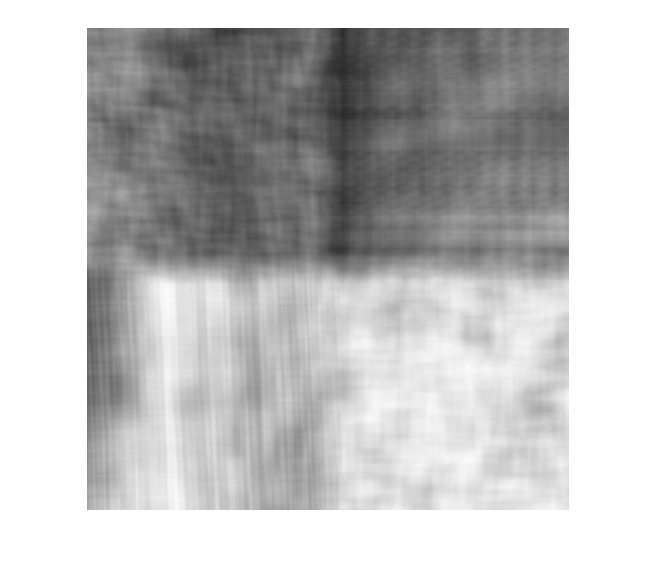
\includegraphics[width=\linewidth]{./images/fi1.png}
    \caption{$\theta$=0}
  \end{subfigure}
  \begin{subfigure}[b]{0.45\linewidth}
    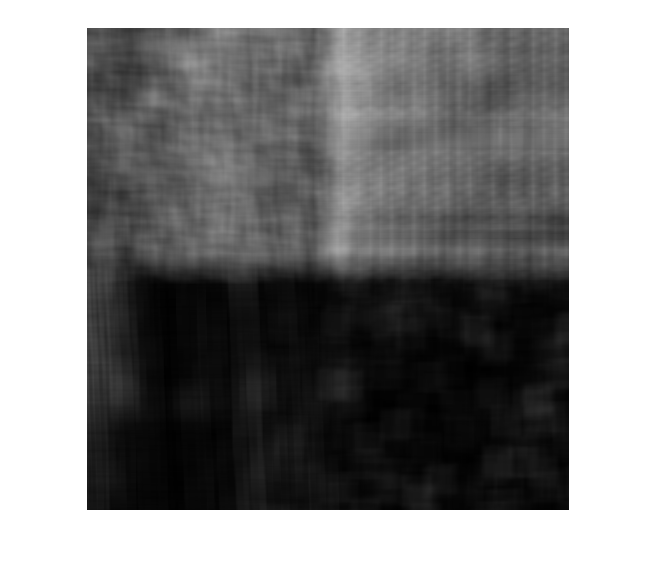
\includegraphics[width=\linewidth]{./images/fi2.png}
    \caption{$\theta$=90}
  \end{subfigure}
  \caption{Feature images for d = 1, $\theta$=0, quadrants q1 and q4.}
  \label{fig:fi0}
\end{figure}
\begin{figure}[h]
  \centering
  \begin{subfigure}[b]{0.45\linewidth}
    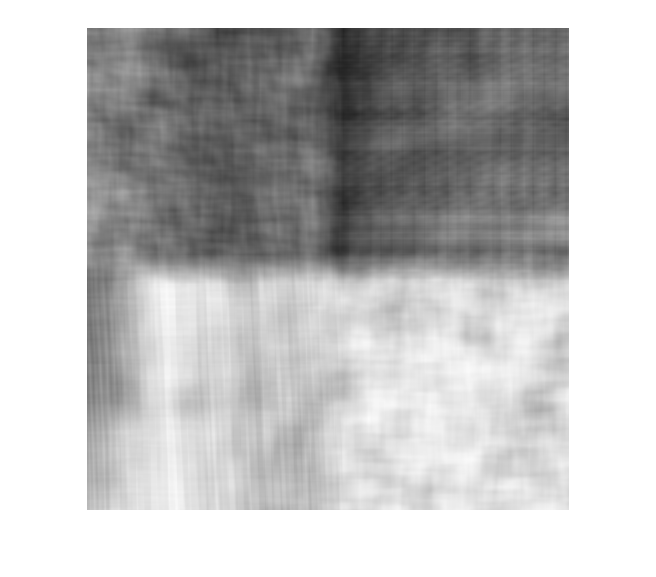
\includegraphics[width=\linewidth]{./images/fi3.png}
    \caption{$\theta$=0}
  \end{subfigure}
  \begin{subfigure}[b]{0.45\linewidth}
    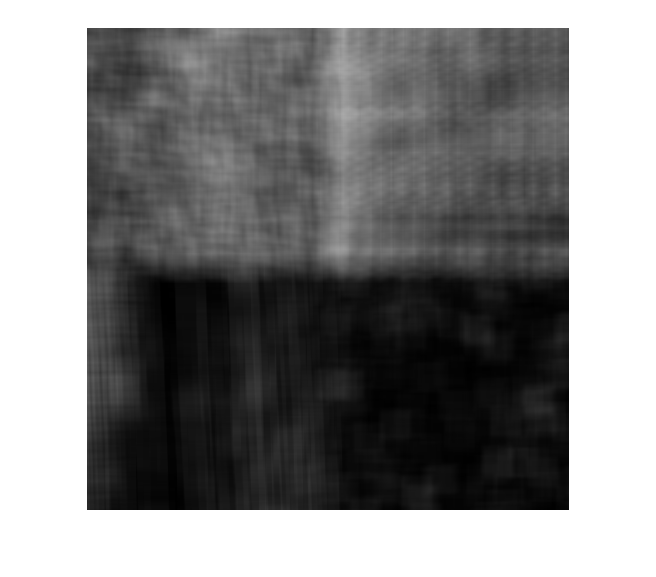
\includegraphics[width=\linewidth]{./images/fi4.png}
    \caption{$\theta$=90}
  \end{subfigure}
  \caption{Feature images for d = 1, $\theta$=90, quadrants q1 and q4.}
  \label{fig:fi90}
\end{figure}

I found it very useful to keep these images in a single matrix structure, so that further calculations were done in a simpler way. We will see the implementation in the next section.

\chapter{Implementing a Gaussian classifier}
To implement the Gaussian classifier, we need to extract more information from the feature images we have gathered so far, namely the mean and covariance matrix for each class. Since we have a training mask, we can use the feature images calculated earlier to determine these values. This is done using the next code, found in \textit{./main.m}:

 \begin{lstlisting}[frame=single]  % Inicia el bloque de código

% Means
mean_v = zeros(num_classes, num_features);
for i = 1:num_features
    auxM = train_img(:,:,i);
    for j = 1:num_classes
        mean_v(j,i) = mean(auxM(train_msk == j));
    end
end
% Cov matrices
cov_mat = zeros(num_features, num_features, num_classes);
for i = 1:num_classes
    cov_mat(:,:,i) = my_cov(train_img, train_msk, nof(i), num_features, i);
end

\end{lstlisting}

The result is a matrix of means, with one element for each class, for each feature image (4x4), and a matrix of covariance matrices using the same principle (4x4x4). We obtained covariance matrices somewhat close to singular, but far enough to invert and use this data. \\
The next task is to actually implement the classifier using this training data. All of the classification was implemented in a single function, in order to use it later on during the testing portion of this project. The formula used to calculate the Gaussian density was the following:\\
\[
p(x|\omega_s) = \frac{1}{(2\pi)^{1/2} |\Sigma_s|^{1/2}}\exp(-\frac{(x-\mu_s)^t\Sigma_s^{-1}(x-\mu_s)}{2})
\]
 The following code was used, also found under \textit{./my\_funcs/my\_mapper.m} (I also added a progress bar for this function because, like the feature extraction, it takes a lot of time to execute):

 \begin{lstlisting}[frame=single]  % Inicia el bloque de código
 
function [ mapped ] = my_mapper( img, mv, cm, n_feat, n_classes )

warning('off','all');
f = waitbar(0,'1','Name','Classifying data...',...
    'CreateCancelBtn','setappdata(gcbf,''canceling'',1)');
setappdata(f,'canceling',0);
[n,m,~] = size(img);
mapped = zeros(n,m);
xv = zeros(1,n_feat);
auxP = zeros(1,n_classes);
step = 0;
steps = n * m;
for i = 1:size(mapped,1)
    for j = 1:size(mapped,2)
        xv(1:n_feat) = img(i,j,:);
        for k = 1:n_classes
            % Gaussian multivariate density
            a = 1/(sqrt(2*pi*abs(det(cm(:,:,k)))));
            auxP(k) = a*exp((-0.5)*(xv-mv(k,:))*(inv(cm(:,:,k)))*(xv-mv(k,:)).');
        end
        if max(auxP) == auxP(1)
            mapped(i,j) = 1;
        elseif max(auxP) == auxP(2)
            mapped(i,j) = 2;
        elseif max(auxP) == auxP(3)
            mapped(i,j) = 3;
        elseif max(auxP) == auxP(4)
            mapped(i,j) = 4;
        end
        step = step + 1;
        if getappdata(f,'canceling')
            break
        end
        waitbar(step/steps,f,sprintf('%.2f',(step/steps)*100))
    end
end
 % Only for beautifying the results (not really necessary)
new_map = zeros(n,m,3);
for i = 1:size(mapped, 1)
    for j = 1:size(mapped, 2)
        if mapped(i,j) == 1
            new_map(i,j,1) = 62/255;
            new_map(i,j,2) = 38/255;
            new_map(i,j,3) = 168/255;
        elseif mapped(i,j) == 2
            new_map(i,j,1) = 39/255;
            new_map(i,j,2) = 151/255;
            new_map(i,j,3) = 235/255;
        elseif mapped(i,j) == 3
            new_map(i,j,1) = 129/255;
            new_map(i,j,2) = 204/255;
            new_map(i,j,3) = 89/255;
        elseif mapped(i,j) == 4
            new_map(i,j,1) = 249/255;
            new_map(i,j,2) = 251/255;
            new_map(i,j,3) = 21/255;
        end
    end
end
delete(f)
map = [62/255, 38/255, 168/255
  39/255, 151/255, 235/255
  129/255, 204/255, 89/255
  249/255, 251/255, 21/255];
figure
imagesc(new_map)
colormap(map)
c = colorbar('Ticks',1/8:1/8:1,'Limits',[0 1],...
         'TickLabels',{'1',' ','2',' ','3',' ','4',' '});
c.Label.String = 'Classes';
title(['Mapped ', img(1:end-4)]);
warning('on','all')
end

\end{lstlisting}

The result of this function is a matrix with a class label for each pixel of the input image. For the training set, the resulting image is shown in \cref{fig:mapped1}.

   \begin{figure}[h]
     \begin{center}
       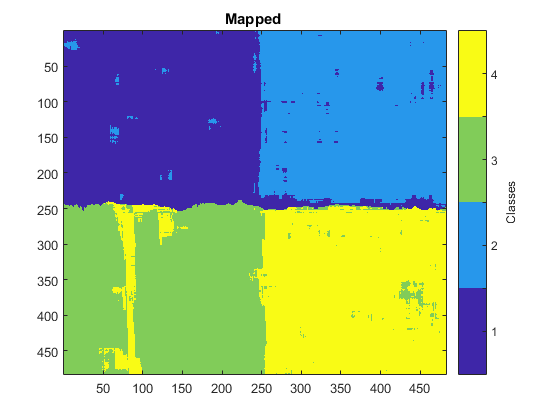
\includegraphics[width=0.5\linewidth]{./images/mapped.png}
     \end{center}
  \caption{Classified training set}
  \label{fig:mapped1}
\end{figure}

\chapter{Training the classifier on the chosen features}
The final training step is to calculate the classification accuracy and the confusion matrix based on the data we'd gathered thus far. As we can see in the classified image, it has done a pretty good job at classifying the textures. I have implemented a function to calculate both the confusion matrix and the error percentage for each class, given by the next code, and found in the file \textit{./my\_funcs/my\_error.m}:

 \begin{lstlisting}[frame=single]  % Inicia el bloque de código

function [ ctv, conf_m ] = my_error( tm, mi )
ctv = zeros(1, 4);
t_test = 0;
t = zeros(1, 4);
e = zeros(1, 4);
conf_m = zeros(4, 4);
for i = 1:numel(tm)
    if tm(i) ~= 0
        t_test = t_test + 1;
        if tm(i) == 1
            t(1) = t(1) + 1;
            if mi(i) ~= 1
                e(1) = e(1) + 1;
                conf_m(1,mi(i)) = conf_m(1,mi(i)) + 1;
            elseif mi(i) == 1
                conf_m(1,1) = conf_m(1,1) + 1;
            end
        elseif tm(i) == 2
            t(2) = t(2) + 1;
            if mi(i) ~= 2
                e(2) = e(2) + 1;
                conf_m(2,mi(i)) = conf_m(2,mi(i)) + 1;
            elseif mi(i) == 2
                conf_m(2,2) = conf_m(2,2) + 1;
            end
        elseif tm(i) == 3
            t(3) = t(3) + 1;
            if mi(i) ~= 3
                e(3) = e(3) + 1;
                conf_m(3,mi(i)) = conf_m(3,mi(i)) + 1;
            elseif mi(i) == 3
                conf_m(3,3) = conf_m(3,3) + 1;
            end
        elseif tm(i) == 4
            t(4) = t(4) + 1;
            if mi(i) ~= 4
                e(4) = e(4) + 1;
                conf_m(4,mi(i)) = conf_m(4,mi(i)) + 1;
            elseif mi(i) == 4
                conf_m(4,4) = conf_m(4,4) + 1;
            end
        else
            tm(i)
        end
    end
end
for i = 1:4
    ctv(i) = (1-(double(e(i))/double(t(i))))*100;
end
end

\end{lstlisting}

The results for these calculations are shown in \cref{tab:ps1} and \cref{tab:cm1}. The overall classification accuracy for the training data, based on this results, is \textbf{96.66\%}.

\begin{table}[H]
    \centering
    \begin{tabular}{ccccc}
        \toprule
        \(\boldsymbol{}\) & \(\boldsymbol{Class 1}\) & \(\boldsymbol{Class 2}\) & \(\boldsymbol{Class 3}\) & \(\boldsymbol{Class 4}\)
        \\
        \midrule
        \textbf{Percentage of success} & 98.7110 & 98.5484 & 91.5953 & 97.6166
	\\
        \bottomrule
    \end{tabular}
    \caption{Success by class}
    \label{tab:ps1}
\end{table}

\begin{table}[H]
    \centering
    \begin{tabular}{ccccc}
        \toprule
        \(\boldsymbol{}\) & \(\boldsymbol{Class 1}\) & \(\boldsymbol{Class 2}\) & \(\boldsymbol{Class 3}\) & \(\boldsymbol{Class 4}\)
        \\
        \midrule
        Class 1 & 44110 & 576 & 0 & 0
	\\
	Class 2 & 625 & 42432 & 0 & 0
	\\
	Class 3 & 0 & 0 & 37653 & 3455
	\\
	Class 4 & 0 & 0 & 887 & 36328
        \\
        \bottomrule
    \end{tabular}
    \caption{Confusion matrix for training data}
    \label{tab:cm1}
\end{table}

\chapter{Classifying the test images}
The same principle was applied on the test sets, with results as good as expected. These sets are images, slightly different from the training image. To do this, we use the same values for means and covariances matrices we have already calculated and run the same function used for training but with these values. The resulting mapped images are shown in \cref{fig:testmapped}. 
\begin{figure}
  \centering
  \begin{subfigure}[b]{0.45\linewidth}
    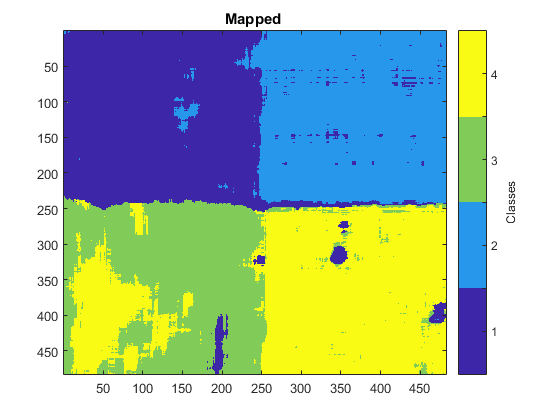
\includegraphics[width=\linewidth]{./images/mapped2.png}
    \caption{mosaic2\_test}
  \end{subfigure}
  \begin{subfigure}[b]{0.45\linewidth}
    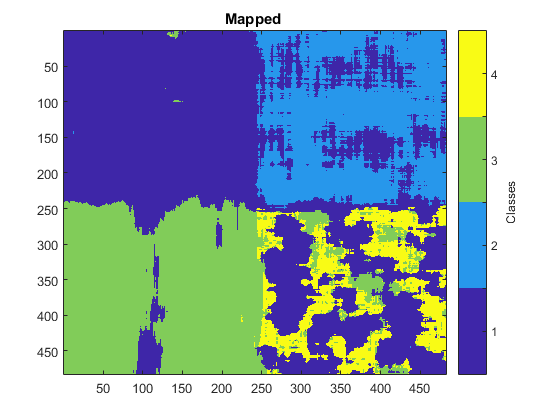
\includegraphics[width=\linewidth]{./images/mapped3.png}
    \caption{mosaic3\_test}
  \end{subfigure}
  \caption{Classified test images.}
  \label{fig:testmapped}
\end{figure}

After classifying these test sets, we can then compute the success rate and the overall classification accuracy, as well as the confussion matrix the same way we did with the training set. The overall classification accuracy for both test data sets is \textbf{89.46\%} and \textbf{75.44\%}, respectively. \cref{tab:ps2} and \cref{tab:cm2} show the results of success score and confusion matrix for \textit{mosaic2\_test}, respectively, and \cref{tab:ps3} and \cref{tab:cm3} show the results for \textit{mosaic3\_test}. \\

\begin{table}[H]
    \centering
    \begin{tabular}{ccccc}
        \toprule
        \(\boldsymbol{}\) & \(\boldsymbol{Class 1}\) & \(\boldsymbol{Class 2}\) & \(\boldsymbol{Class 3}\) & \(\boldsymbol{Class 4}\)
        \\
        \midrule
        \textbf{Percentage of success} & 98.1896 & 97.7518 & 65.1333 & 96.2542
	\\
        \bottomrule
    \end{tabular}
    \caption{Success by class for mosaic2\_test}
    \label{tab:ps2}
\end{table}

\begin{table}[H]
    \centering
    \begin{tabular}{ccccc}
        \toprule
        \(\boldsymbol{}\) & \(\boldsymbol{Class 1}\) & \(\boldsymbol{Class 2}\) & \(\boldsymbol{Class 3}\) & \(\boldsymbol{Class 4}\)
        \\
        \midrule
        Class 1 & 43877 & 807 & 2 & 0
	\\
	Class 2 & 968 & 42089 & 0 & 0
	\\
	Class 3 & 796 & 0 & 26775 & 13537
	\\
	Class 4 & 632 & 6 & 756 & 35821
        \\
        \bottomrule
    \end{tabular}
    \caption{Confusion matrix for for mosaic2\_test}
    \label{tab:cm2}
\end{table}

\begin{table}[H]
    \centering
    \begin{tabular}{ccccc}
        \toprule
        \(\boldsymbol{}\) & \(\boldsymbol{Class 1}\) & \(\boldsymbol{Class 2}\) & \(\boldsymbol{Class 3}\) & \(\boldsymbol{Class 4}\)
        \\
        \midrule
        \textbf{Percentage of success} & 99.9262 & 72.4226 & 92.9162 & 30.2163
	\\
        \bottomrule
    \end{tabular}
    \caption{Success by class for mosaic3\_test}
    \label{tab:ps3}
\end{table}

\begin{table}[H]
    \centering
    \begin{tabular}{ccccc}
        \toprule
        \(\boldsymbol{}\) & \(\boldsymbol{Class 1}\) & \(\boldsymbol{Class 2}\) & \(\boldsymbol{Class 3}\) & \(\boldsymbol{Class 4}\)
        \\
        \midrule
        Class 1 & 44653 & 6 & 27 & 0
	\\
	Class 2 & 11874 & 31183 & 0 & 0
	\\
	Class 3 & 2911 & 0 & 38196 & 1
	\\
	Class 4 & 21965 & 3 & 4002 & 11245
        \\
        \bottomrule
    \end{tabular}
    \caption{Confusion matrix for mosaic3\_test}
    \label{tab:cm3}
\end{table}


\printbibliography
\end{document}
